\chapter{20-Time, Revolutions}

\section{Question 1}

`In this exercise you can decide what to do next on your game:3 This time, though, it can only be a
novel feature (not code quality improvement or similar).
Define your requirements and get them approved by your teaching assistant. The implementation
and process will be based on the same criteria used for the working version, plus it will take into
account whether you use design patterns and advanced object-oriented programming.' \\

The final thing we wanted to add to our game, was a boss. The boss has to have the ability to shoot the player. To make this boos harder to kill we gave the boss a few lives. Now when you have completed all the normal levels, the boss level appears, and when you kill the boss you win the game.

\section{Question 2}

`During the analysis and design phases of this extension use responsibility driven design and UML
(push to the repository the single PDF file including all the documents produced).'

\subsection{Introduction}

For the FinalEnemy we had to create two new classes, 'FinalEnemy' and 'BubbleEnemy', both these classes are related to other classes.

\subsection{Responsibility Driven Design} 

\subsubsection{FinalEnemy}
\textit{Responsibility:} \\
The final enemy has to be able to move from the top to the bottom of the screen, and it has to be able to shoot a BubbleEnemy. When the player hits the final enemy with it's bubble, he has to lose a life. \\ \\
\textit{Collaborations:} \\
FinalEnemy collaborates with Observable to be able to send updates to Observer classes. It also collaborates with  the SpriteBase, to get the x and y, and with both the Bubble extendsions, to fire bubbles and to be shot by bubbles.

\subsubsection{BubbleEnemy}
\textit{Responsibility:} \\
The BubbleEmey's are shot by the FinalEnemy, these bubbles have the ability to move through walls. When one of these bubbles hits the player, the player has to die. \\ \\
\textit{Collaborations:} \\
BubbleEnemy collaborates with Observable to be able to send updates to Observer classes. It also collaborates with  the SpriteBase, to get the x and y, with the FinalEnemy to be shot by, and with the Player to kill.

\subsection{UML}
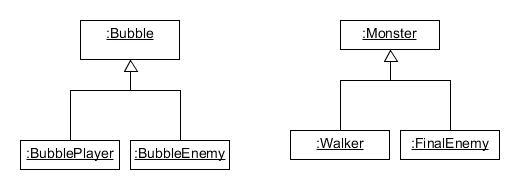
\includegraphics[width=150mm]{FinalEnemyUml.png}